\documentclass{project}
\usepackage[pdfauthor={L Jones},pdftitle={Software Engineering Group Project, IDesign Specification},pdftex]{hyperref}
\usepackage{graphicx}
\usepackage[export]{adjustbox}
\graphicspath{ {images} }
\begin{document}
\title{Software Engineering Group Project}
\subtitle{Design Specificaion}
\author{L. Jones, T. Oram, T. Garapasi, M. Goly, W. Jones, A. Neaves, J. Mir, T. MIlls}     
\shorttitle{Design Specification}
\version{1.5}
\status{Rview}
\date{2015-11-24}
\configref{SE-12-DS}
\maketitle
\tableofcontents
\newpage
\section{INTRODUCTION}
\subsection{Purpose of this document}
The purpose of this document is to outline the ways in which our systems work and communicate with one another, explain how users will interact with the system as a whole and to provide a basic user-interface design for TaskerMAN and TaskerCLI.
\subsection{Scope}
This document specifically covers the Deployment Description and Interaction Design sections of the Design Specifications Standards \cite{se.qa.ds}, and as such does not include the Component Description, Significant Classes or Detailed Design sections required of the full Design Specifications Standards.\\
\newline
This document should be read by all project members. It is assumed that the reader is already familiar with the Design Specification Standards \cite{se.qa.ds}.
\subsection{Objectives}
The objectives of this document are as follows:
\begin{itemize}
	\item Explain the way the systems interact with one another and the platforms in which they operate with the asisstance of UML diagrams.
	\item Provide detail on the way in which "actors" are expected to interact with the system through the use of use-case diagrams.
	\item Present a basic User-Interface design for the TaskerMAN and TaskerCLI systems with the aid of images to demonstrate how such systems will operate and keep to the requirements set in the Requirements Specification \cite{se.qa.rs}.
\end{itemize} 
\clearpage
\section{DEPLOYMENT DESCRIPTION}
\subsection{Applications in the system}
The deployment UML diagram below illustrates the division of the software 
system into separate applications and the platforms on which they will be
deployed. \\
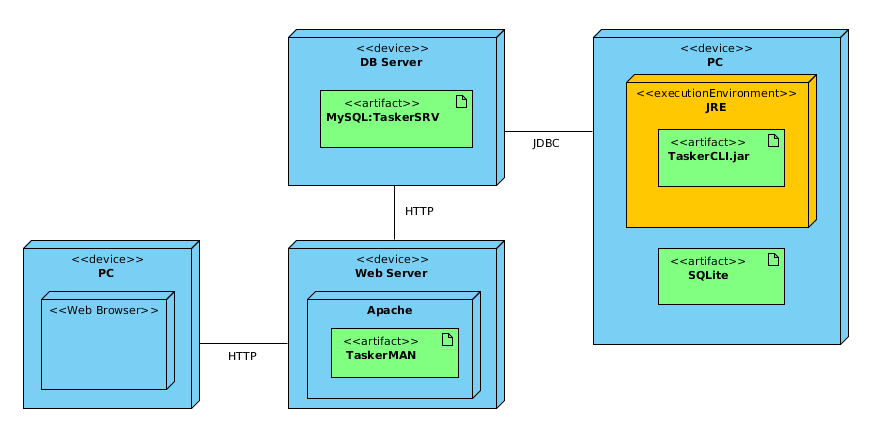
\includegraphics[width=\textwidth]{images/4.1/DeploymentDiagram} \\
The whole system will be composed of the following three components:
\begin{itemize}
	\item TaskerSRV (Database)
	\item TaskerMAN (Web Client)
	\item TaskerCLI (Desktop Client)
\end{itemize} 
TaskerSRV will be deployed onto a database server with a pre-installed MySQL
engine. It will store the critical data of the whole system and make it
accessible to both web and desktop clients through the specified protocols.
TaskerMAN will be deployed as a PHP web application onto an Apache web server
and it will be accessible from the Internet by any client with an installed web 
browser. Finally, TaskerCLI will be a desktop application written in Java, and it
will be deployed as a runnable jar onto a machine running the Java Runtime
Environment. Following the requirements specification\cite{se.qa.rs fr8 local storage}, TaskerCLI will have to
operate both on-line and off-line. Therefore it will have a direct access to 
a local storage provided by the SQLite database.
\subsection{Applications interface}
Unlike the deployment diagram above, the component diagram below depicts the interaction of different modules or components of the proposed system. There are four major components that form the entire system. Only a black box view is shown here. This means that the components are not further decomposed to reveal the inner components. The opposite of this is a white box view which shows not only the major component but also the inner components that form the big picture. 
According to the design specification standard[1], only the simple black box view application interaction is relevant for now. A rundown of the actual interactions is as follows: \\
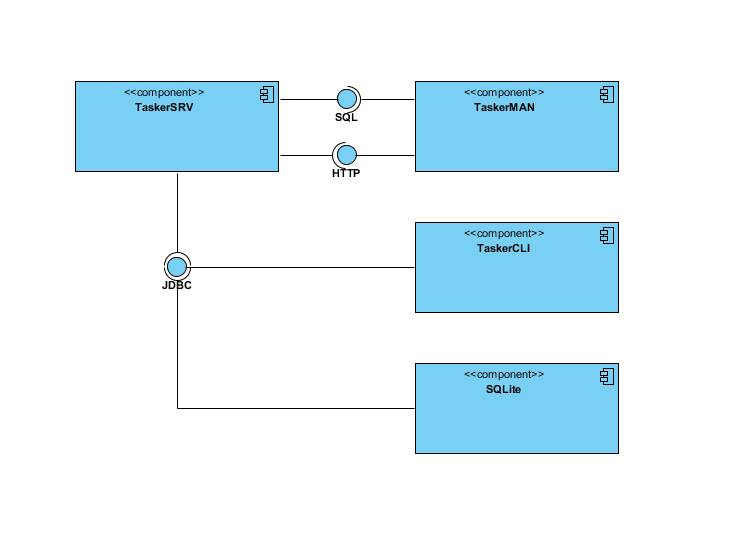
\includegraphics[width=\textwidth]{images/4.2/ApplicationsInterface} 
TaskerSRV - This component, representing the database, consists of one provided interface (solid circle) and two required interfaces (cup shaped). These are:
\begin{itemize}
	\item SQL(provided interface) : Provides an SQL interface, making it possible for the web application, TaskerMAN, to manipulate the database and carry the necessary operations outlined in the requirements[2] such as adding, editing, deleting users or tasks. 
	\item HTTP (required interface): Without the HTTP protocol the database would not be accessed by the TaskerMAN and no operation can take place.
	\item JDBC (required interface): The interface is required so that communication to the SQL can be established and give the required services to the client.
\end{itemize}
TaskerMAN - This component, representing the web application has one required interface (SQL) and one provided interface (HTTP). Without SQL provided by TaskerSRV, TaskerMAN will not be able to do anything. It will remain a useless dummy. Also if it can not provide the HTTP communication interface then it would not be able to access the database. \\
\newline 
TaskerCLI - This component representing the client has one provided interface (JDBC). Since it is using Java to connect to the database, TaskerSRV as well as SQLite will require that the interface JDBC be implemented on the client�or else there will be no database connection. \\
\newline SQLite - This component representing the local database on the client has one required interface (JDBC) which makes it possible for the client to connect to it.
\section{INTERACTION DESIGN}
\subsection{Use-cases}
\subsubsection{TaskerMAN Use-Case}
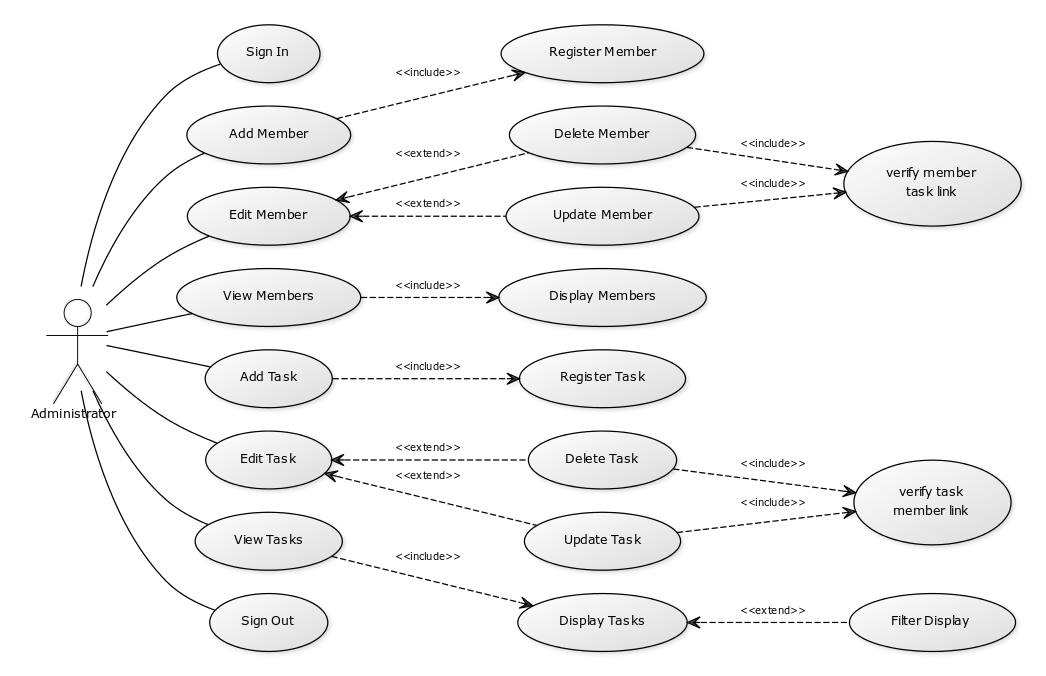
\includegraphics[width=\textwidth]{images/5.1/TaskerMANUseCase}
The TaskerMAN use case diagram above depicts clearly how the web administration application will be able to be used by the administrator.  The necessary functions depicted in the specification requirements\cite{se.qa.rs} are clearly accessible to the administrator after logging into the system. These functionalities are, add task, edit task, view tasks, filter display, add and edit member. The options update member and delete members as well as update task and delete task are labelled as extending.  This is because they are options and an administrator may or may not choose to delete a task or member.  Also they include a verification so that the administrator might be aware, for example, that a member to be deleted or updated might be currently assigned a task or vice versa.  Similarly the filter display is extended since an administrator may choose to filter display results or not.
Example usage scenario:
\begin{enumerate}
	\item The administrator logs onto the web application system.
	\item Selects "add member" and registers the members.
	\item Administrator clicks on "view members" to make sure the members are added.
	\item Administrator realises that a member name was misspelled. He or she clicks on "edit member" and selects the option "update member".  Necessary updates are done.
	\item Administrator then clicks on "add task" and a necessary form is displayed where data is entered.
	\item Administrator decides that the task was allocated to the wrong member.  He or she clicks on "edit task".  An appropriate page is loaded where the task can be selected and a reallocation can be carried out.
	\item Administrator decides that one more task is actually not needed.  He or she clicks on "edit task", selects the task and clicks on "delete task".  A prompt is displayed informing that the task is associated with a member.  If the administrator is comfortable to delete, then the action is executed.
	\item Administrator clicks on "view tasks" and all the tasks displayed.  An option is also available for the administrator to filter display results accordingly as specified in the requirements[8].
	\item The administrator has finished using the system and he or she clicks on "log out" and the session ends.
\end{enumerate}
\subsubsection{TaskerCLI Use-Case}
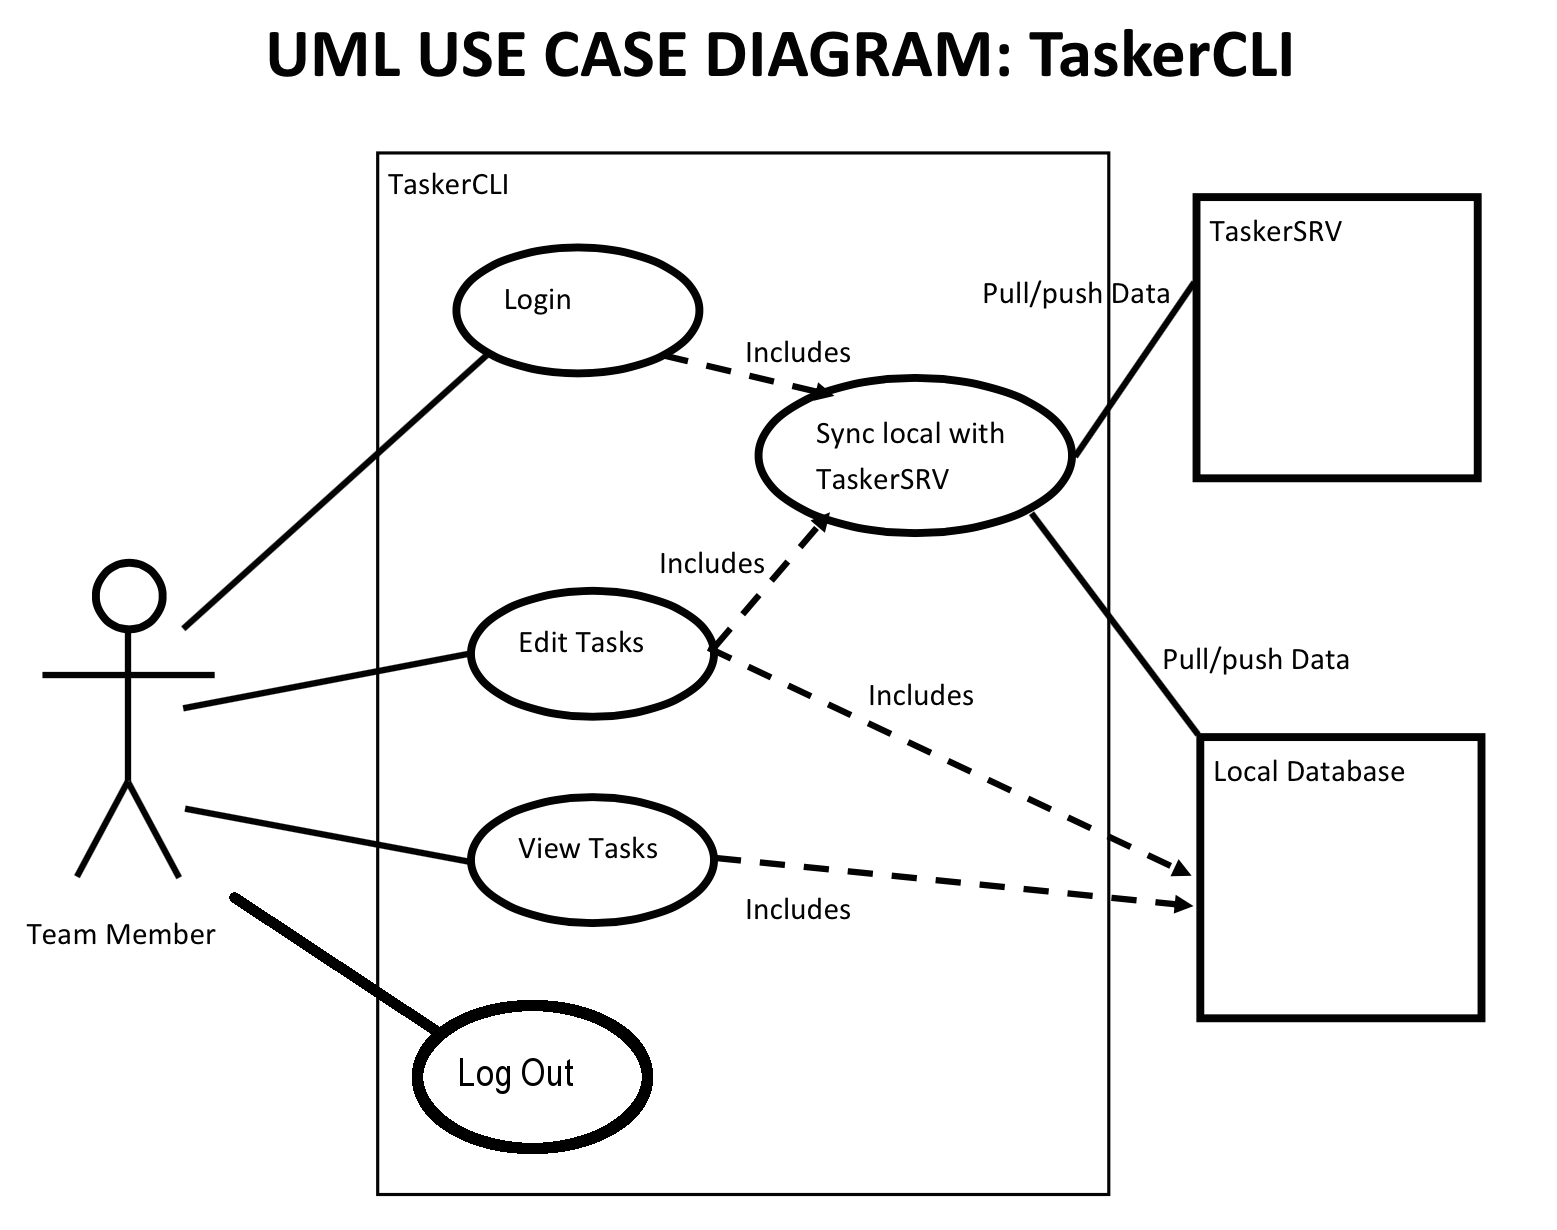
\includegraphics[width=\textwidth]{images/5.1/TaskerCLIUseCase}
The TaskerCLI use-case diagram above depicts how TaskerCLI will be used by "actors".  The diagram illustrates the different functions the application must contain as outlined in the requirements specification \cite{se.qa.rs}. These are user identification (login), local storage of tasks, task synchronisation and the function to edit tasks, both locally and to TaskerSRV. Example usage scenario:
\begin{enumerate}
	\item The actor logs onto the Java application.
	\item The application synchronises with TaskerSRV and pulls the tasks assigned to the actor and stores them to the SQLite database.
	\item The actor clicks on 'View Task' and the task information is loaded from the SQLite database and displayed on-screen.
	\item The actor confirms changes and clicks 'Edit Task', this will trigger another synchronisation to occur, and the changes will be pushed to TaskerSRV and to the SQLite database.
	\item The user has completed their actions and clicks 'Log Out', terminating the system.
\end {enumerate}	
\subsection{User Interface design}
\subsubsection{TaskerMAN Interface Design} 
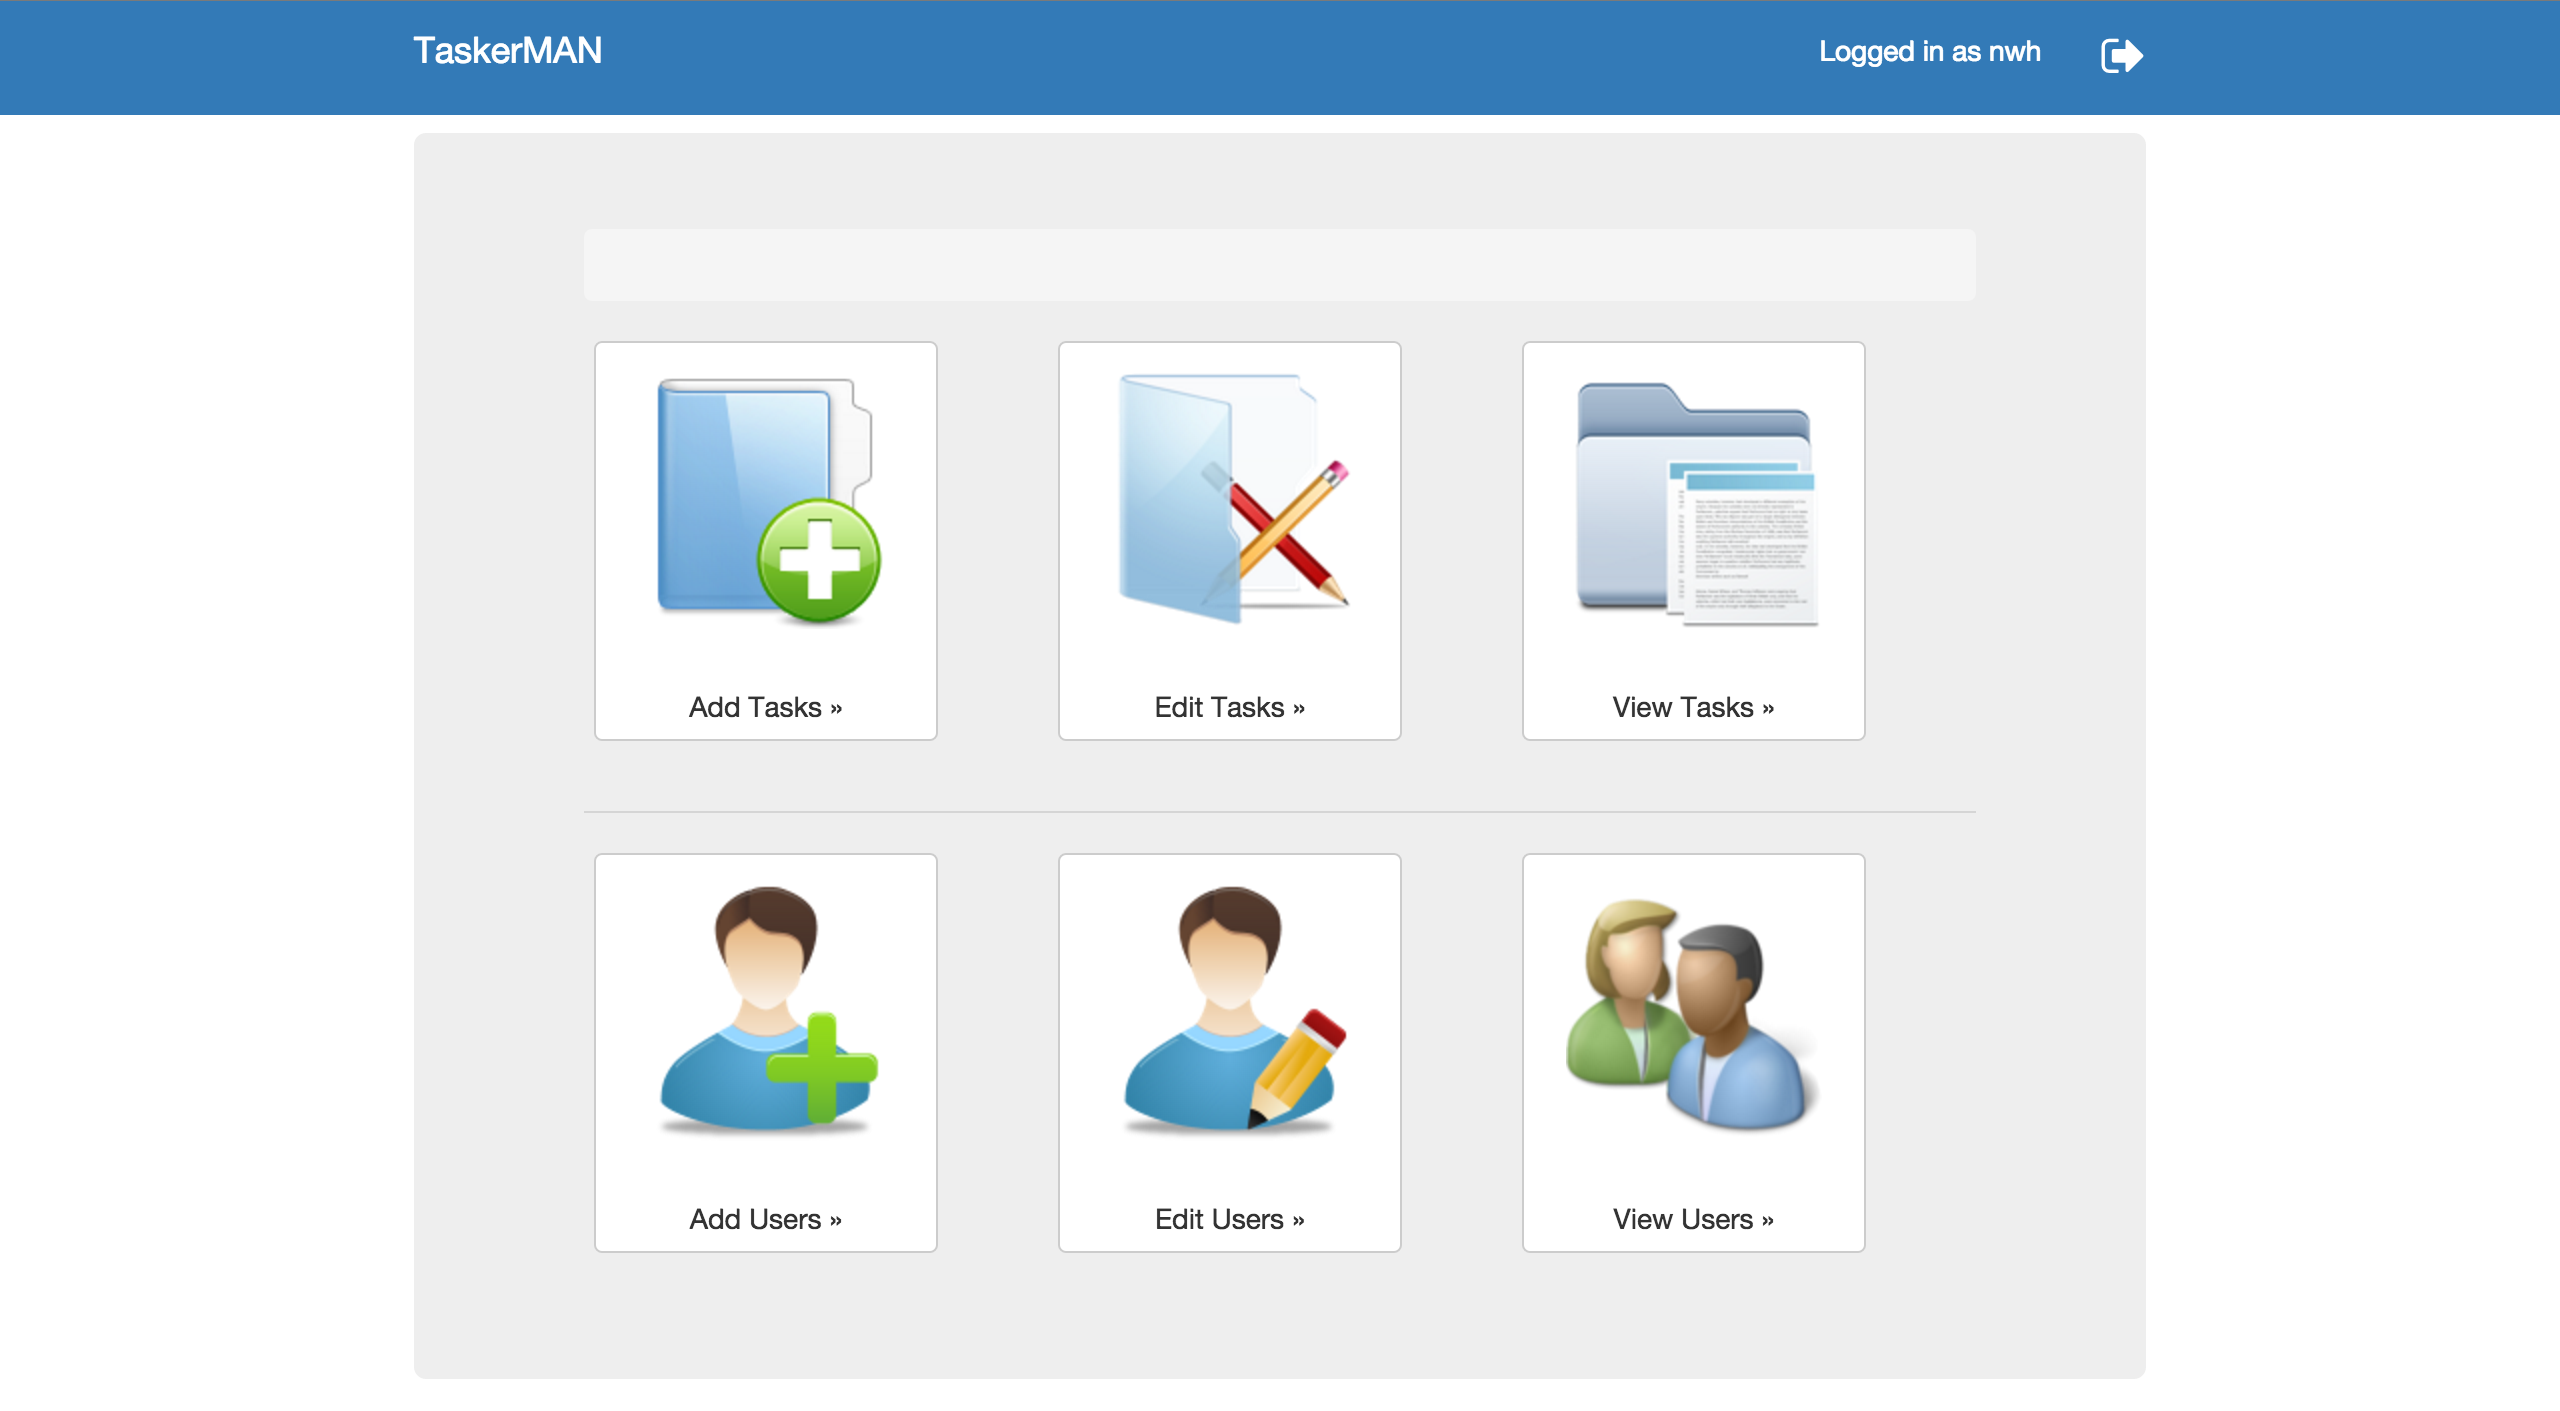
\includegraphics[width=0.75\textwidth, center]{images/5.2/TaskerMANHomePage} \\
This is the home page of the web interface, it is very easy to use and presents you with six options which provides very quick access to all aspects of the Tasker. To begin we will click on the 'Add User' button. This will re-direct us to the 'Add Team Member' page. \\~\\
\newline
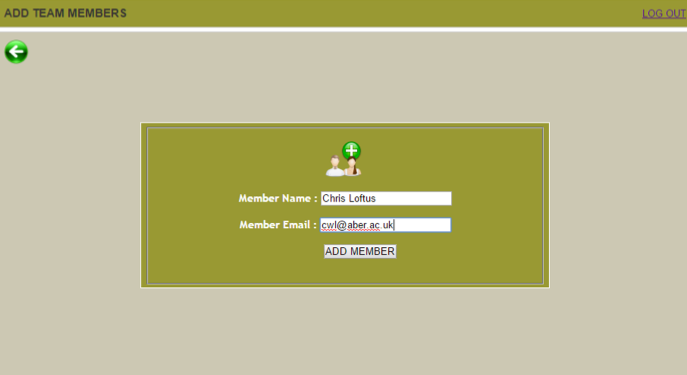
\includegraphics[width=0.75\textwidth, center]{images/5.2/TaskerMANAddUser} \\
Here within the 'Add Team Member' page you will be presented with the form above which then enables you to create a user by presenting their name and e-mail. Upon pressing the 'Add member' button the new member will be added to the database as required \cite{se.qa.rs fr3}. Clicking on the 'backwards arrow' in the top-left corner allows users to return to the home page. In fact the 'backwards arrow' exists within all of the sites internal pages and serves the same function of returning to the home page. \\~\\
\newline
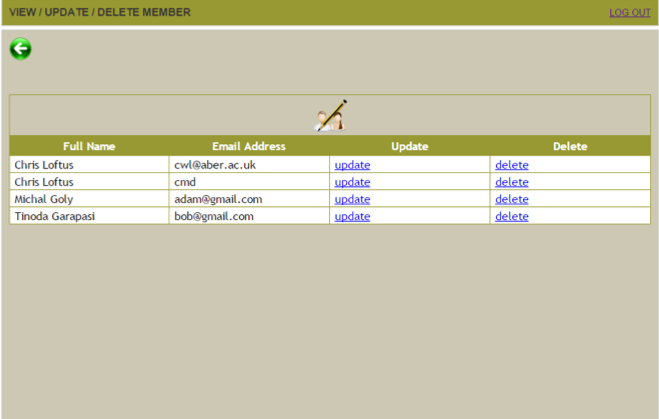
\includegraphics[width=0.75\textwidth, center]{images/5.2/TaskerMANEditUser} \\
To update or delete user data as required \cite{se.qa.rs fr3} click on the 'Edit User' button from the home page and you will be presented with this page, displaying users' names, e-mail addresses and options to update/delete, clicking 'update' re-directs to a page with the same interface as the 'Add Team Member' page where name and e-mail can be updated, clicking 'delete' will prompt the user to verify with a 'confirm'/'cancel' option that they are sure they want to proceed, before re-directing them to a page confirming their deletion and a delete command will be submitted to the database to remove the user from the database. \\~\\
\newline
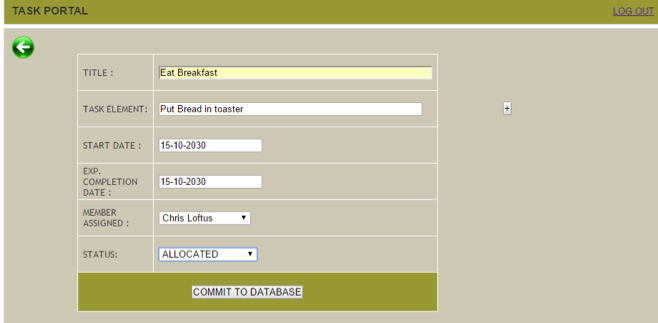
\includegraphics[width=0.75\textwidth, center]{images/5.2/TaskerMANAddTask} \\
Clicking 'Add Task' from the home page will re-direct to the task portal, This is where people can make tasks which will then be submitted to specific users \cite{se.qa.rs fr4}. This task portal layout will also be used when updating tasks. 'Title' and 'Title Description' will be text boxes for user input, 'Start Date' and 'End Completion Date' are currently also text boxes, however to improve validation we may add a drop down calendar at both dates. The 'Member's Assigned' box contains a drop-down list of all the members currently added so it makes it easy to assign or re-assign people to specific tasks \cite{se.qa.rs fr5}. 'Status' is also a drop-down list that can be changed between 'Allocated', 'Abandoned' \cite{se.qa.rs fr6}, 'Completed' and 'Not allocated'. The commit to database button then adds the task to the database and will then sync up with the client, a confirmation screen is then shown to show the user that the task has been successfully added. \\~\\
\newline
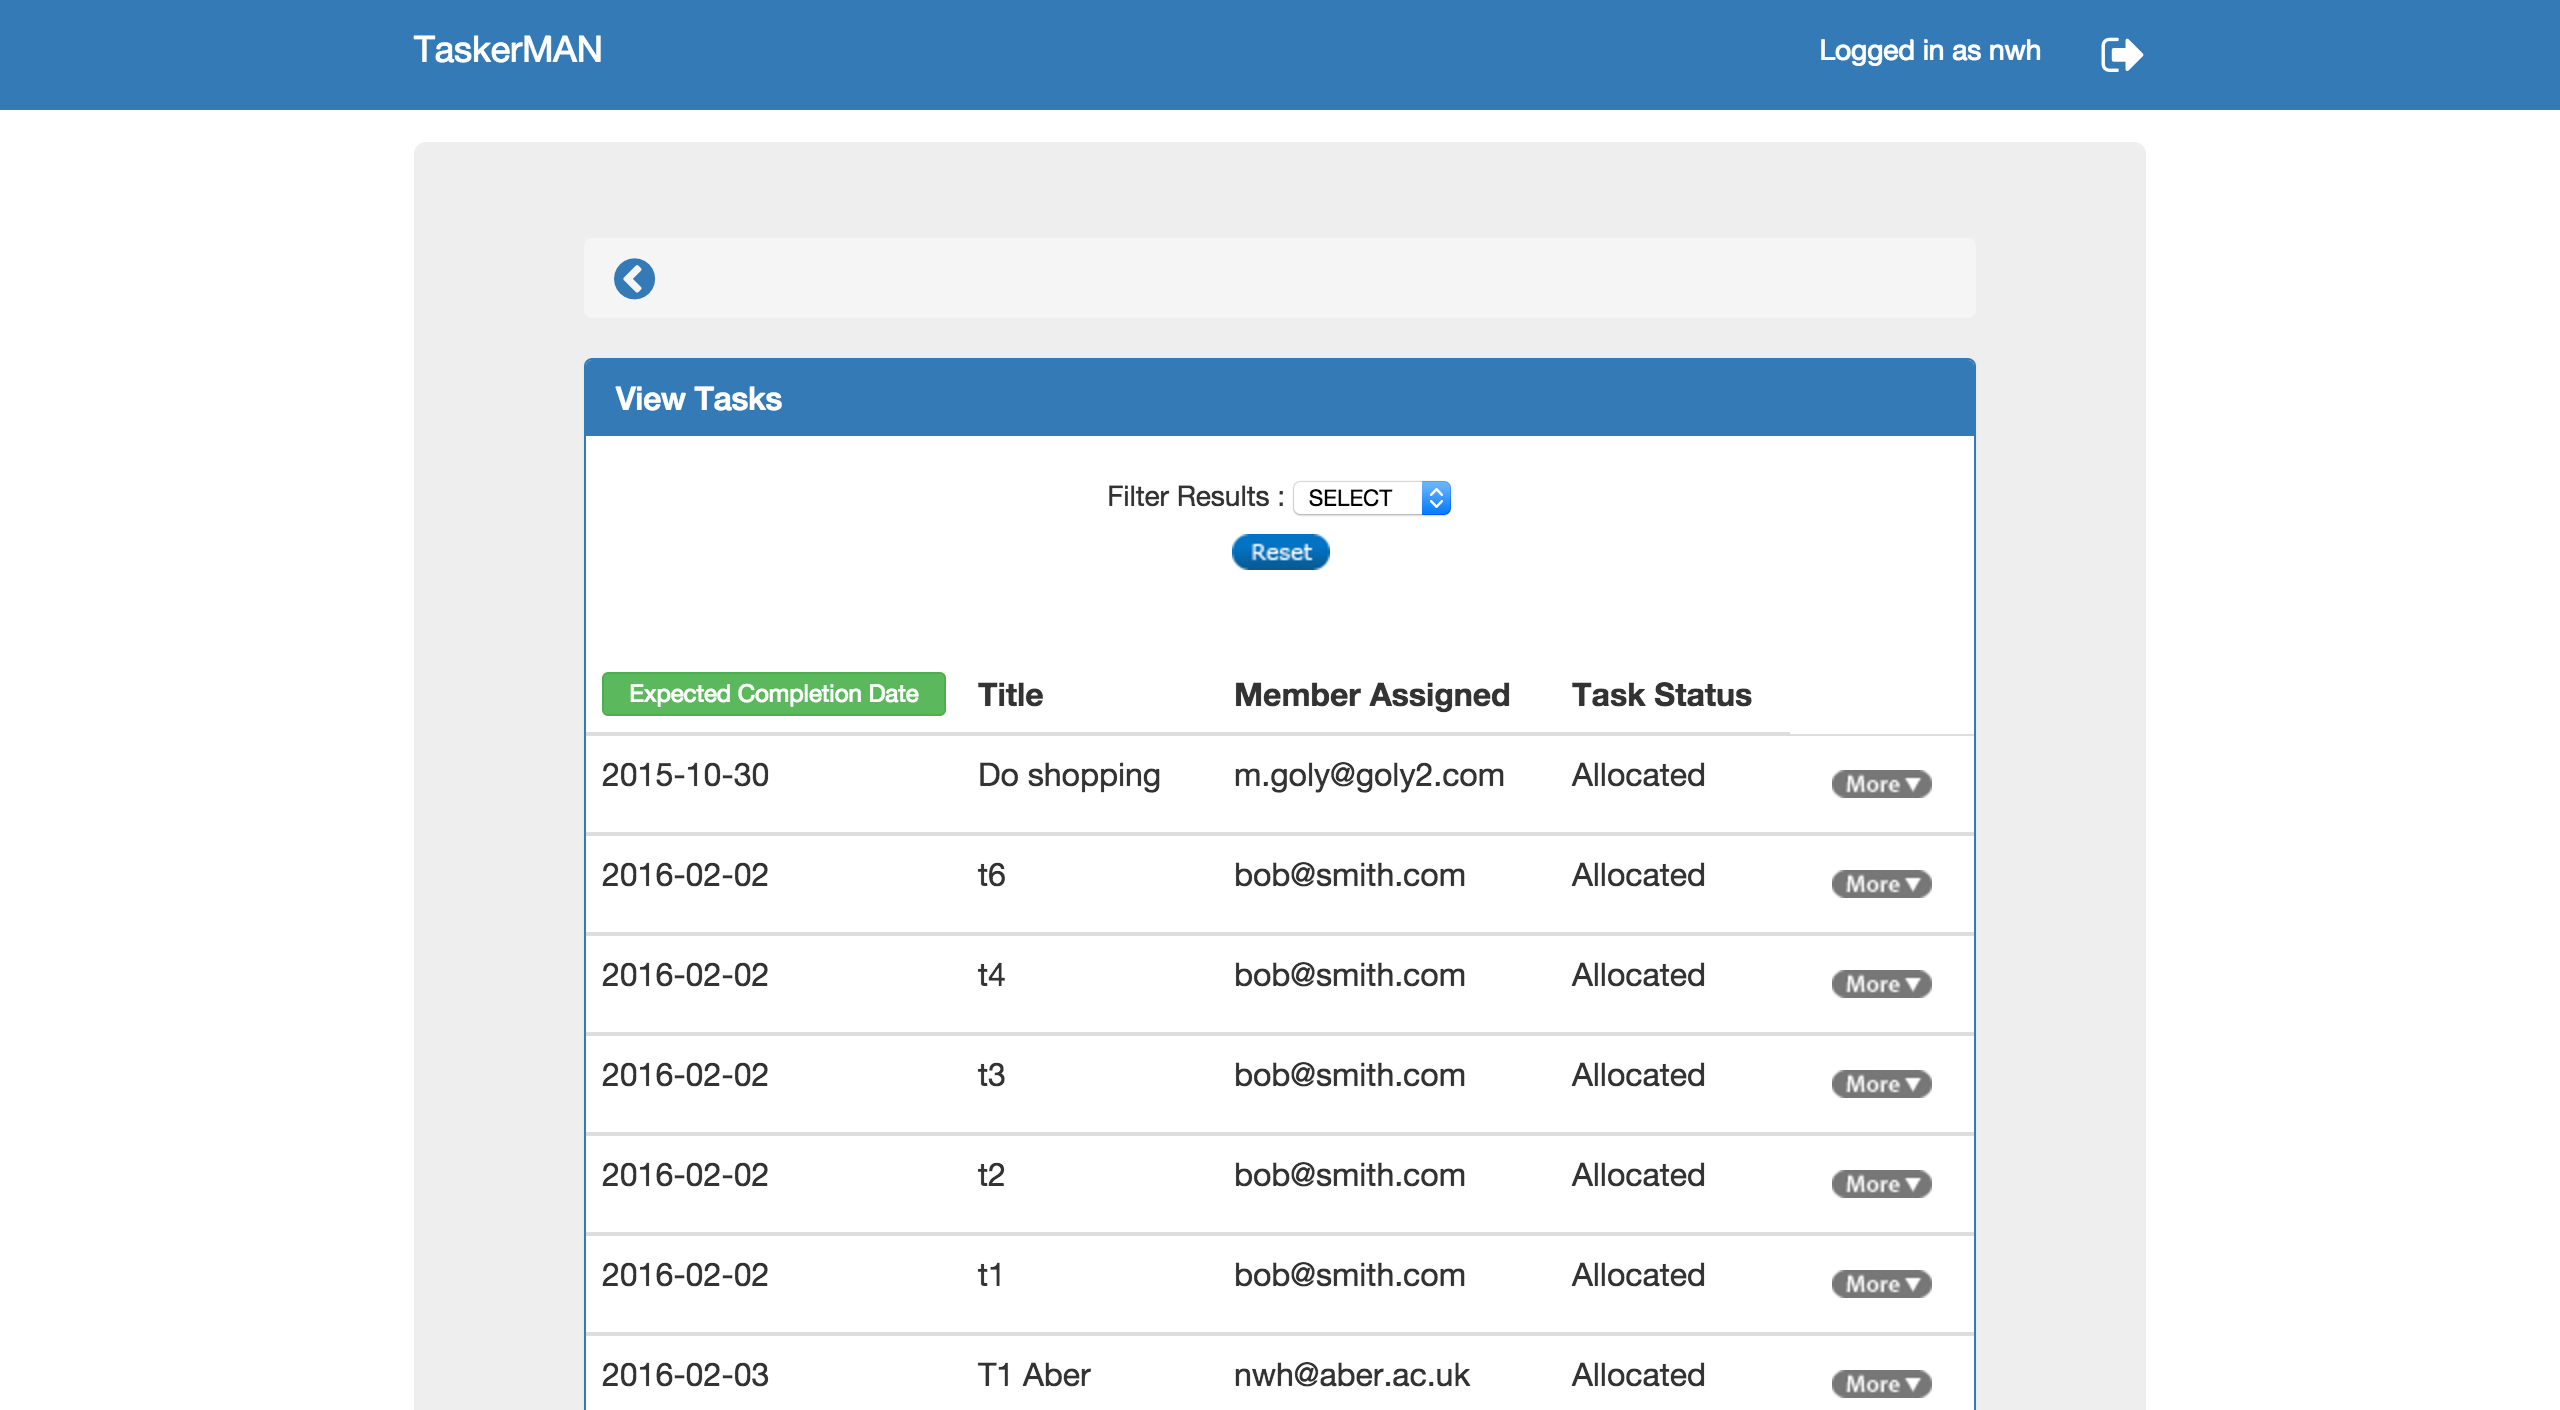
\includegraphics[width=0.75\textwidth, center]{images/5.2/TaskerMANViewTask} \\
To view tasks from the home page the 'view tasks' button must be clicked. This page shows all of the tasks that have been made, you can filter them by using the drop-down box at the top. This list os sorted by expected completion date by default \cite{se.qa.rs fr7}.
\subsubsection{TaskerCLI Interface Design} 
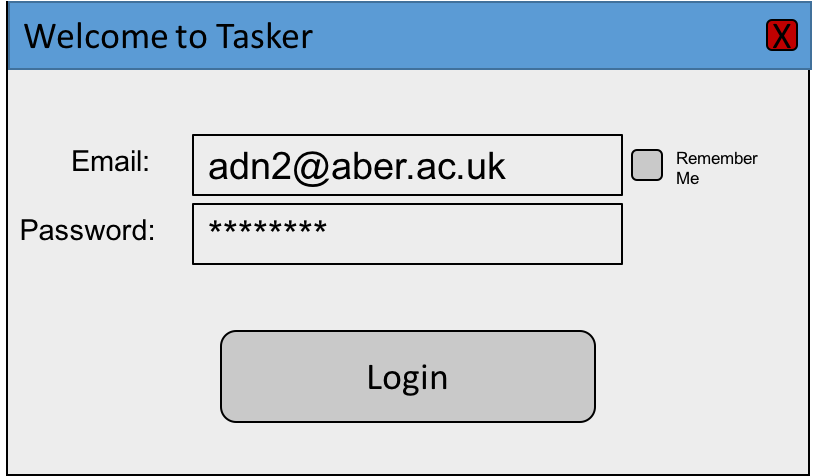
\includegraphics[width=0.5\textwidth, center]{images/5.2/TaskerCLILogin} \\
The login screen, the first screen to appear when the client loads. TaskerCLI does not synchronise with the database until the user has logged in as specified in Requirements Specifications.\cite{se.qa.rs fr8 user id} \\~\\
\newline
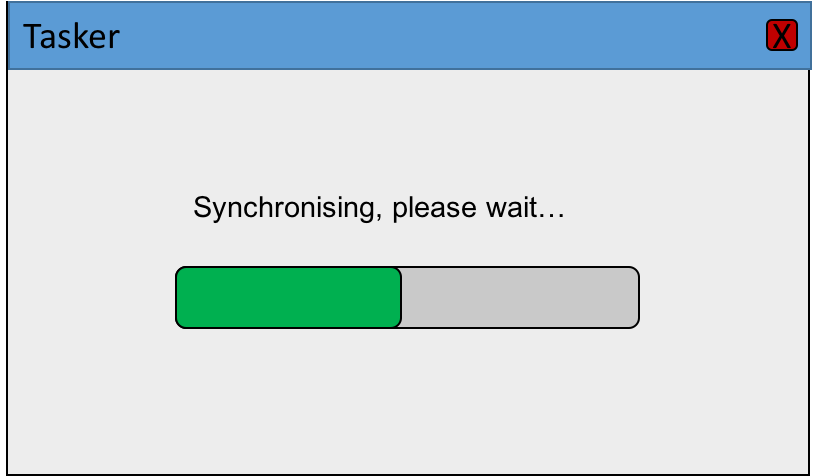
\includegraphics[width=0.5\textwidth, center]{images/5.2/TaskerCLILoading} \\
The synchronisation screen occurs between the login and main client page. As per the requirements specifications \cite{se.qa.rs fr11} this screen will also occur before and after local editing if network access is available, as well as occurring every 5 minutes by default should no local editing take place. This will display the relevant information from the database as it's downloading the data. Ideally this will be a fast enough task that this screen should be seen for as little time as possible. \\~\\
\newline
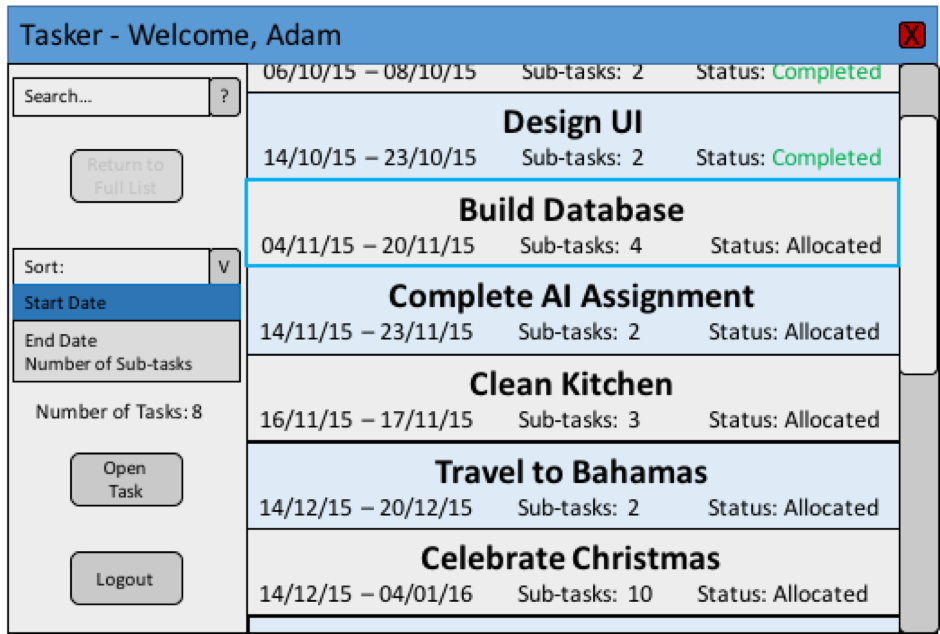
\includegraphics[width=0.75\textwidth, center]{images/5.2/TaskerCLIMainScreen} \\
The 'Main Screen' of TaskerCLI. It shows a list of tasks assigned to the person who signed in, as well as options for sorting and searching through the list. Clicking on the 'Log Out' button will re-direct the user back to the login authentication screen. Double clicking a task's panel, or selecting a task and clicking the 'open task' button shows more detail about the task \cite{se.qa.rs fr10}, as well as the editable parts, such as the completed/allocated attribute and the sub-task list comments. In this example we'll double-click on the "Build Database" task. \\~\\
\newline
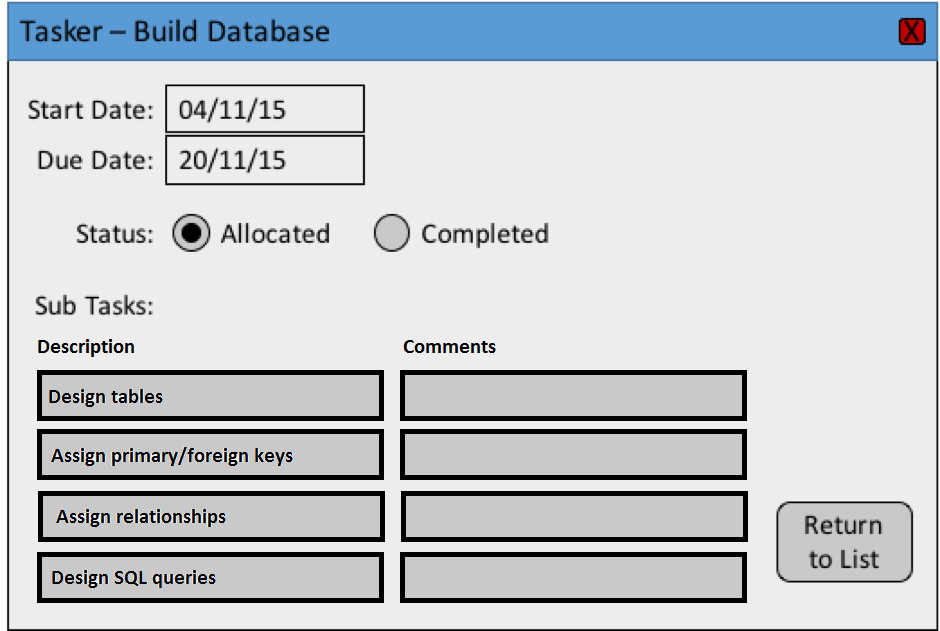
\includegraphics[width=0.75\textwidth, center]{images/5.2/TaskerCLITaskInfo} \\
This screen shows more details about the "Build Database". It displays all the task's information and allows the user to edit task step comments and change task's status \cite{se.qa.rs fr10}. \\~\\
\newline
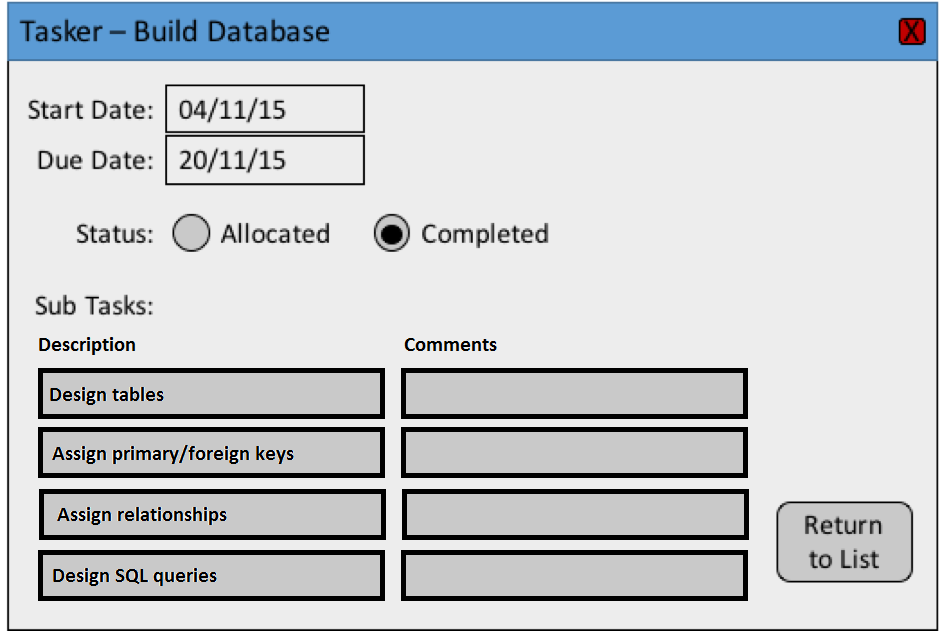
\includegraphics[width=0.75\textwidth, center]{images/5.2/TaskerCLITaskUpdated} \\
In this image we've changed the status to 'Completed'. We can press the 'Return to List' button to return to the 'Main Screen'. Doing so will prompt the synchronisation screen to appear and an attempt will be made to connect to the network and update the information on the remote MySQL database. If unsuccessful the user will still be re-directed back to the 'Main Screen', however the client will be now operating locally using the local SQLite database until a connection with the MySQL can be re-established.\\~\\
\newline
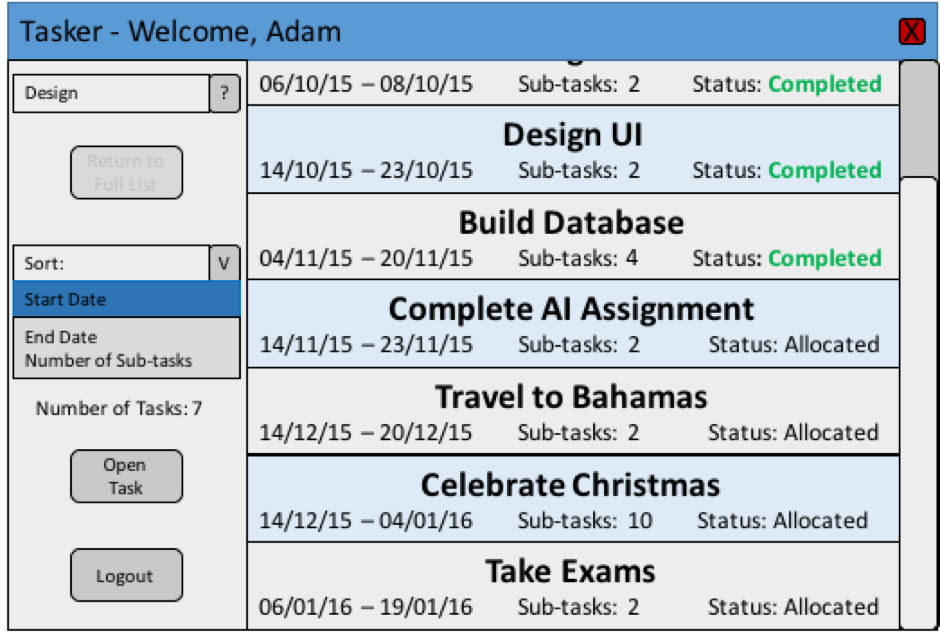
\includegraphics[width=0.75\textwidth, center]{images/5.2/TaskerCLIMainScreenUpdated} \\
Note the changes made are now reflected in this list. Also note that the task named 'Clean Kitchen' has disappeared. This is something that could happen if said task were marked 'Abandoned' via TaskerMAN while the user was editing a task within TaskerCLI, provided there is a network connection. \\~\\
\newline
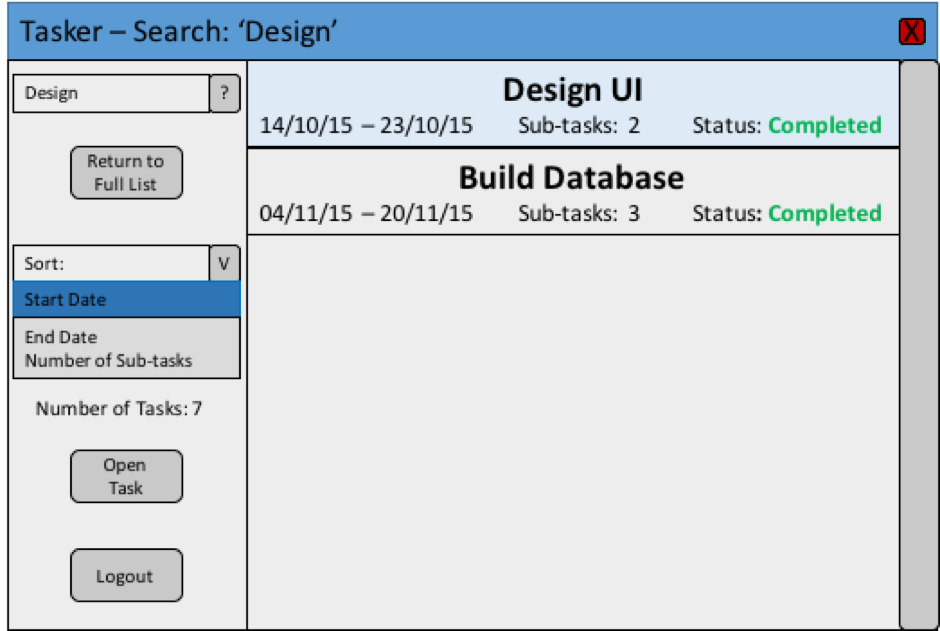
\includegraphics[width=0.75\textwidth, center]{images/5.2/TaskerCLIMainScreenSearch} \\
Searching using the text box searches for the string provided in the task's name, and/or it's sub-tasks. Also note that the 'return to full list' button is only selectable if there is currently a search parameter in the search box.\\~\\
\newline
There is a large focus on designing the interfaces of both TaskerCLI and TaskerMAN to be intuitive to regular computer users \cite{se.qa.rs ir1}.
\section{Component Description}
\section{Significant Classes}
\subsection{TaskerCLI Significant Classes}
\subsection{TaskerMAN Significant Classes}
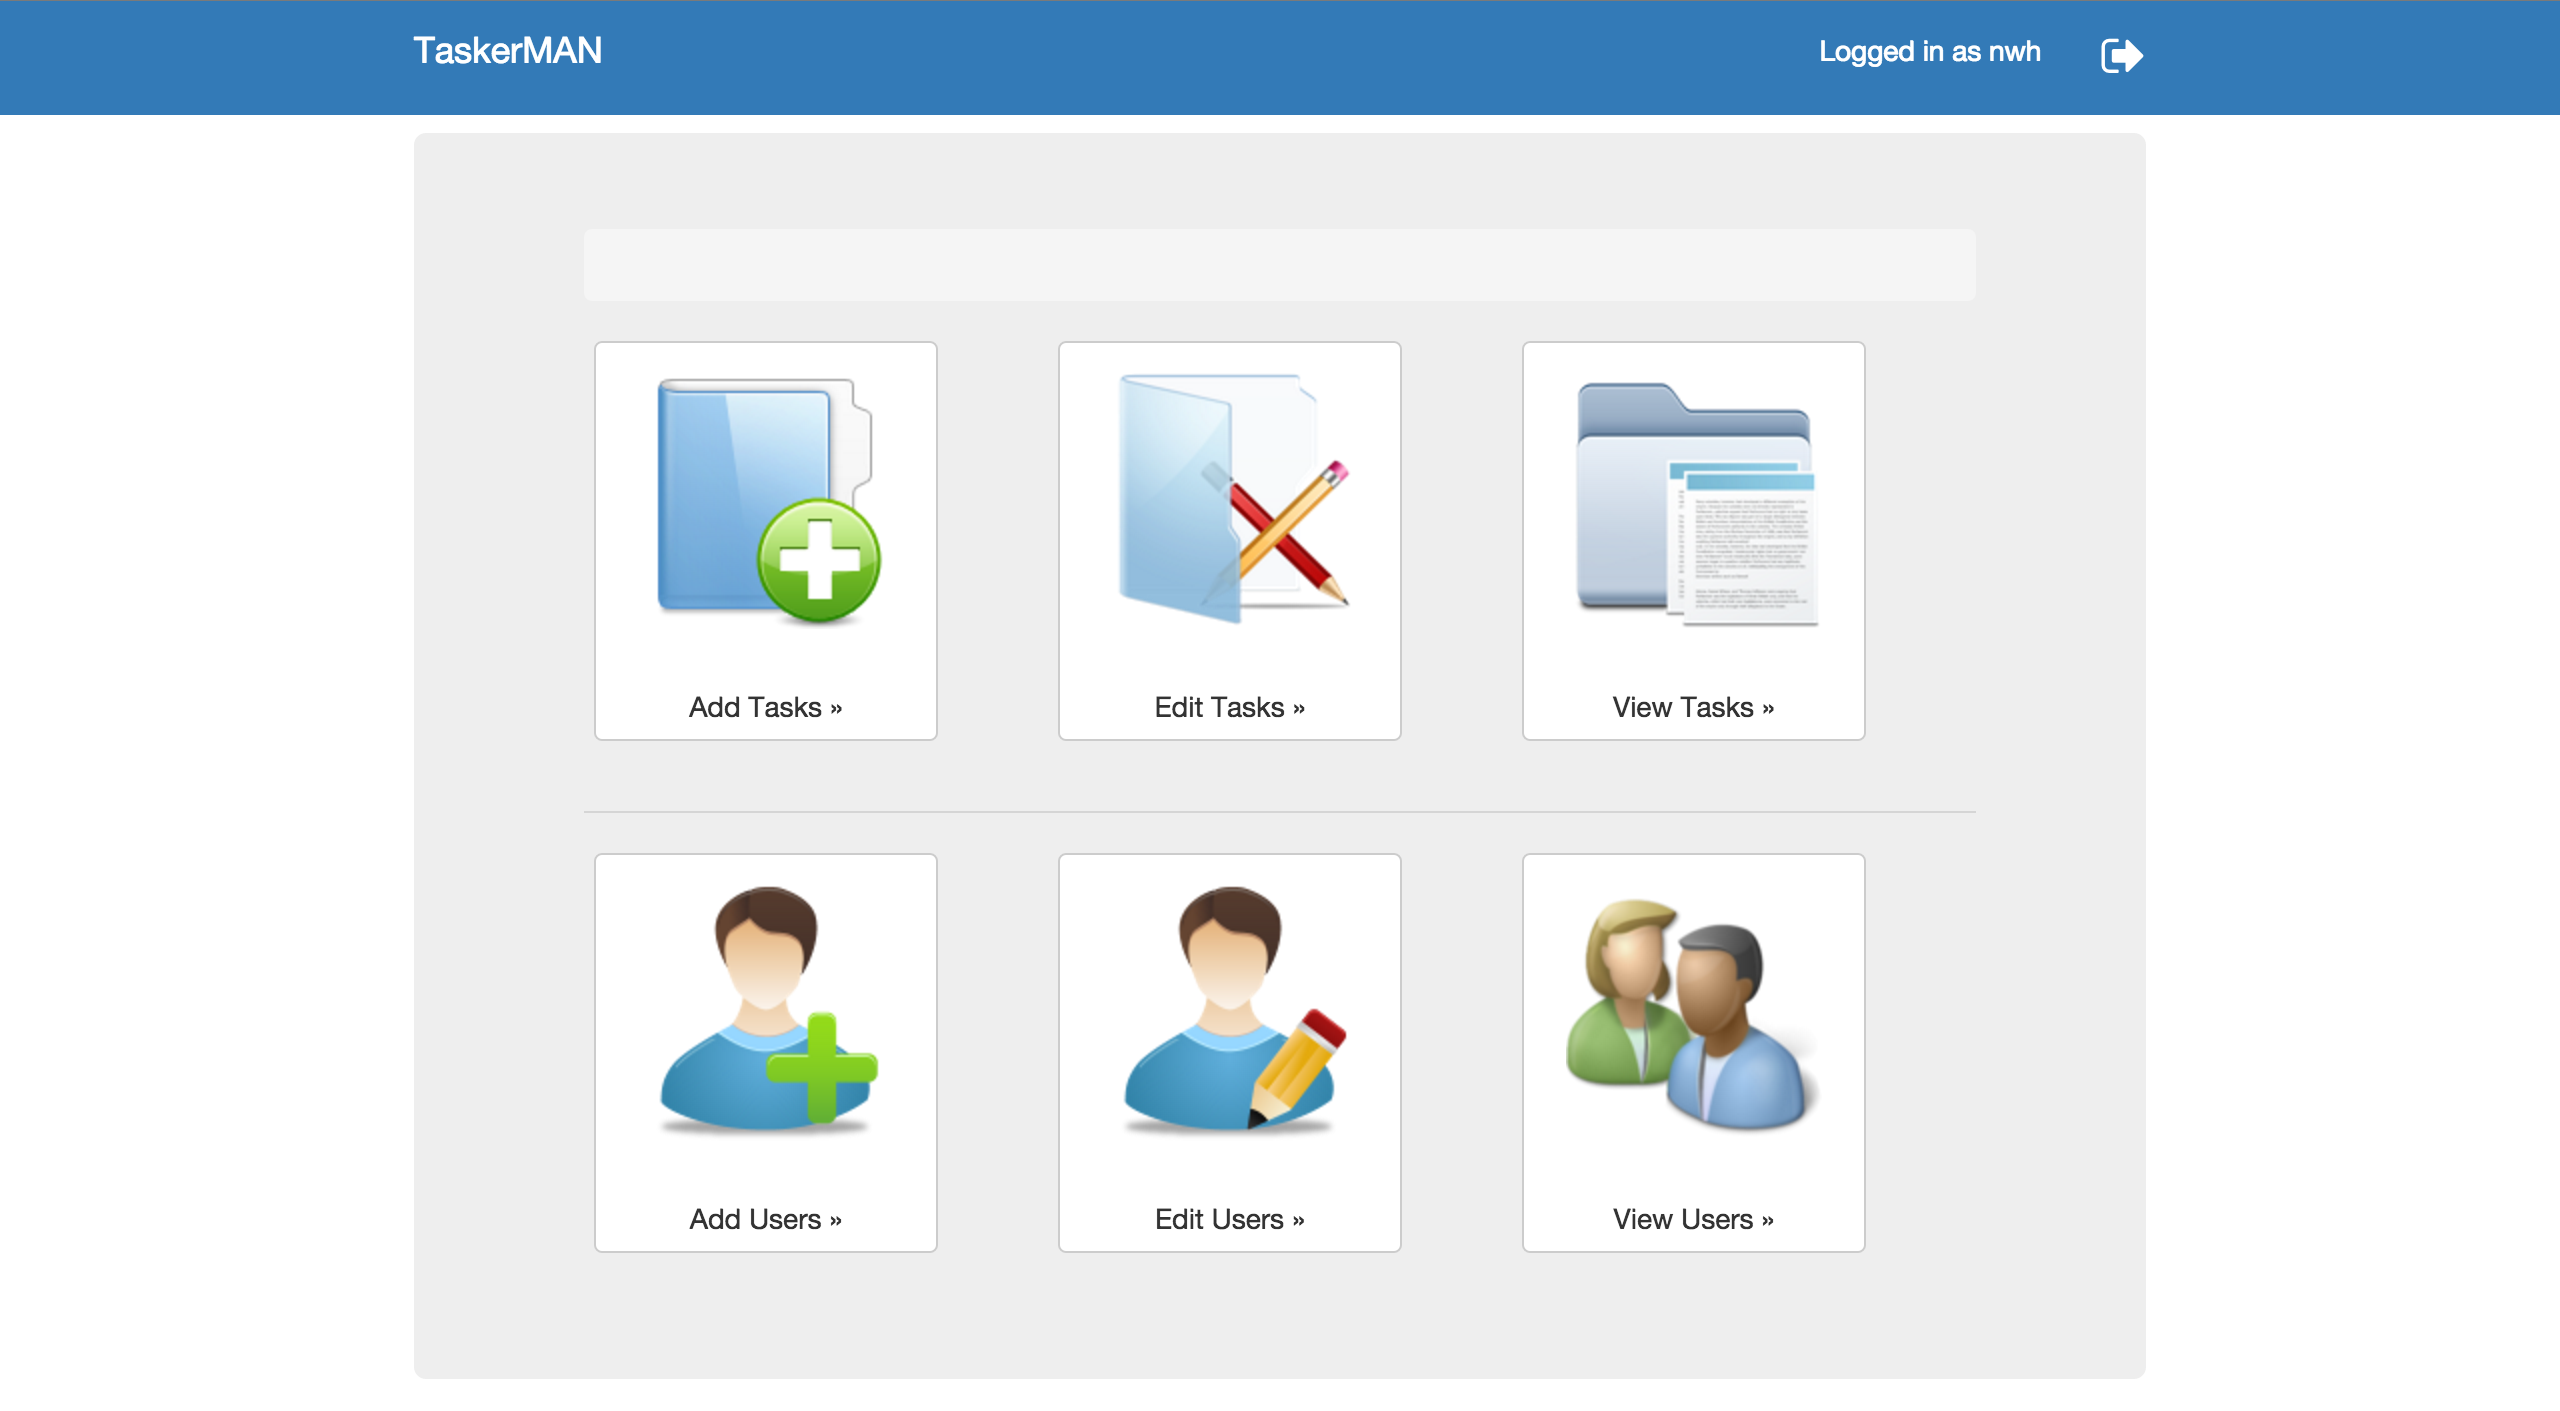
\includegraphics[width=0.75\textwidth, center]{images/5.2/TaskerMANHomePage} \\
This is the home page of the web interface, it is very easy to use and presents you with six options which provides very quick access to all aspects of the Tasker. \\~\\
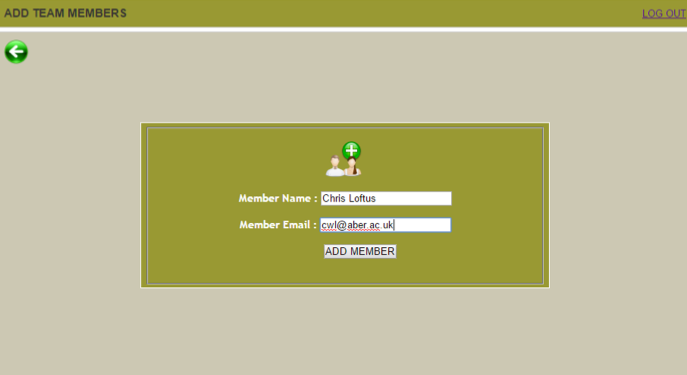
\includegraphics[width=0.75\textwidth, center]{images/5.2/TaskerMANAddUser} \\
If you click on the add user button you will be presented with the form above which then enables you to create a user just by presenting their name and email. We intend to have some sort of email validation to give authentication to users. Once the ?Add member? button is clicked, the new member will be added to the database. The main navigation on this page is just if you want to leave the page you click the arrow in the top left hand side of the page which will take you back to the home page (this is the same on all the pages).  Once you have added a member, a confirmation screen will come up which gives you 3 options, you can return to the home page by pressing the arrow button, add another user by clicking the hyperlink in the middle of page or logout. \\~\\
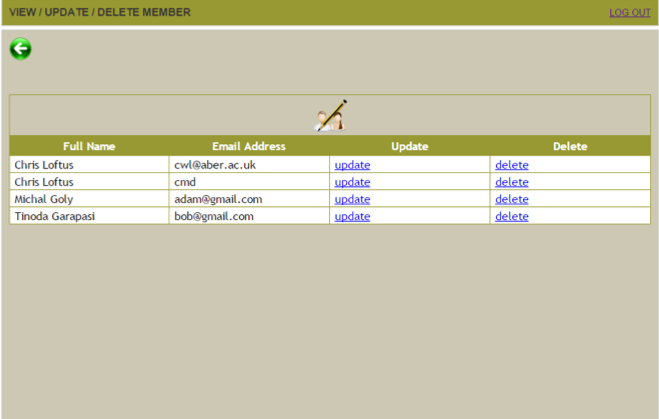
\includegraphics[width=0.75\textwidth, center]{images/5.2/TaskerMANEditUser} \\
The screen above presents you with all the users on the system, here you can change their details such as their names and emails, or by deleting them. Once the delete button is pressed a delete command will be submitted to the database to remove the user from the database. The navigation here is once again very simple, you have an arrow in the top left that takes you back to the home screen and a logout button. \\~\\
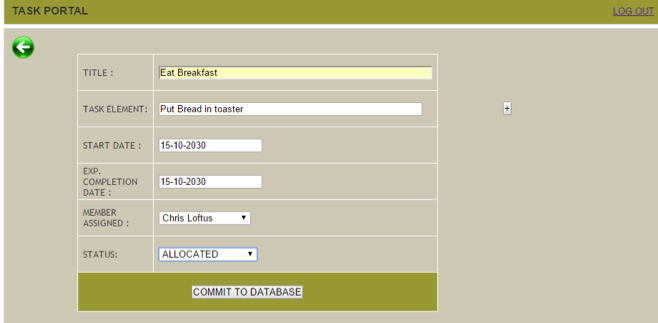
\includegraphics[width=0.75\textwidth, center]{images/5.2/TaskerMANAddTask} \\
This is where people will make tasks which will then be submitted to specific users. To improve validation we may add a drop down calendar to the start and end date. The member?s assigned box contains a drop down list of all the members you have added so it makes it easy to assign people to specific tasks. Then the status of that task can be changed from allocated, abandoned, completed and not allocated. The commit to database button then adds the task to the database and will then sync up with the client, a confirmation screen is then shown to show the user that the task has been successfully added. The + at task element lets you add more than one element to the task so for example enables you to add sub tasks or break the task down further. \\~\\
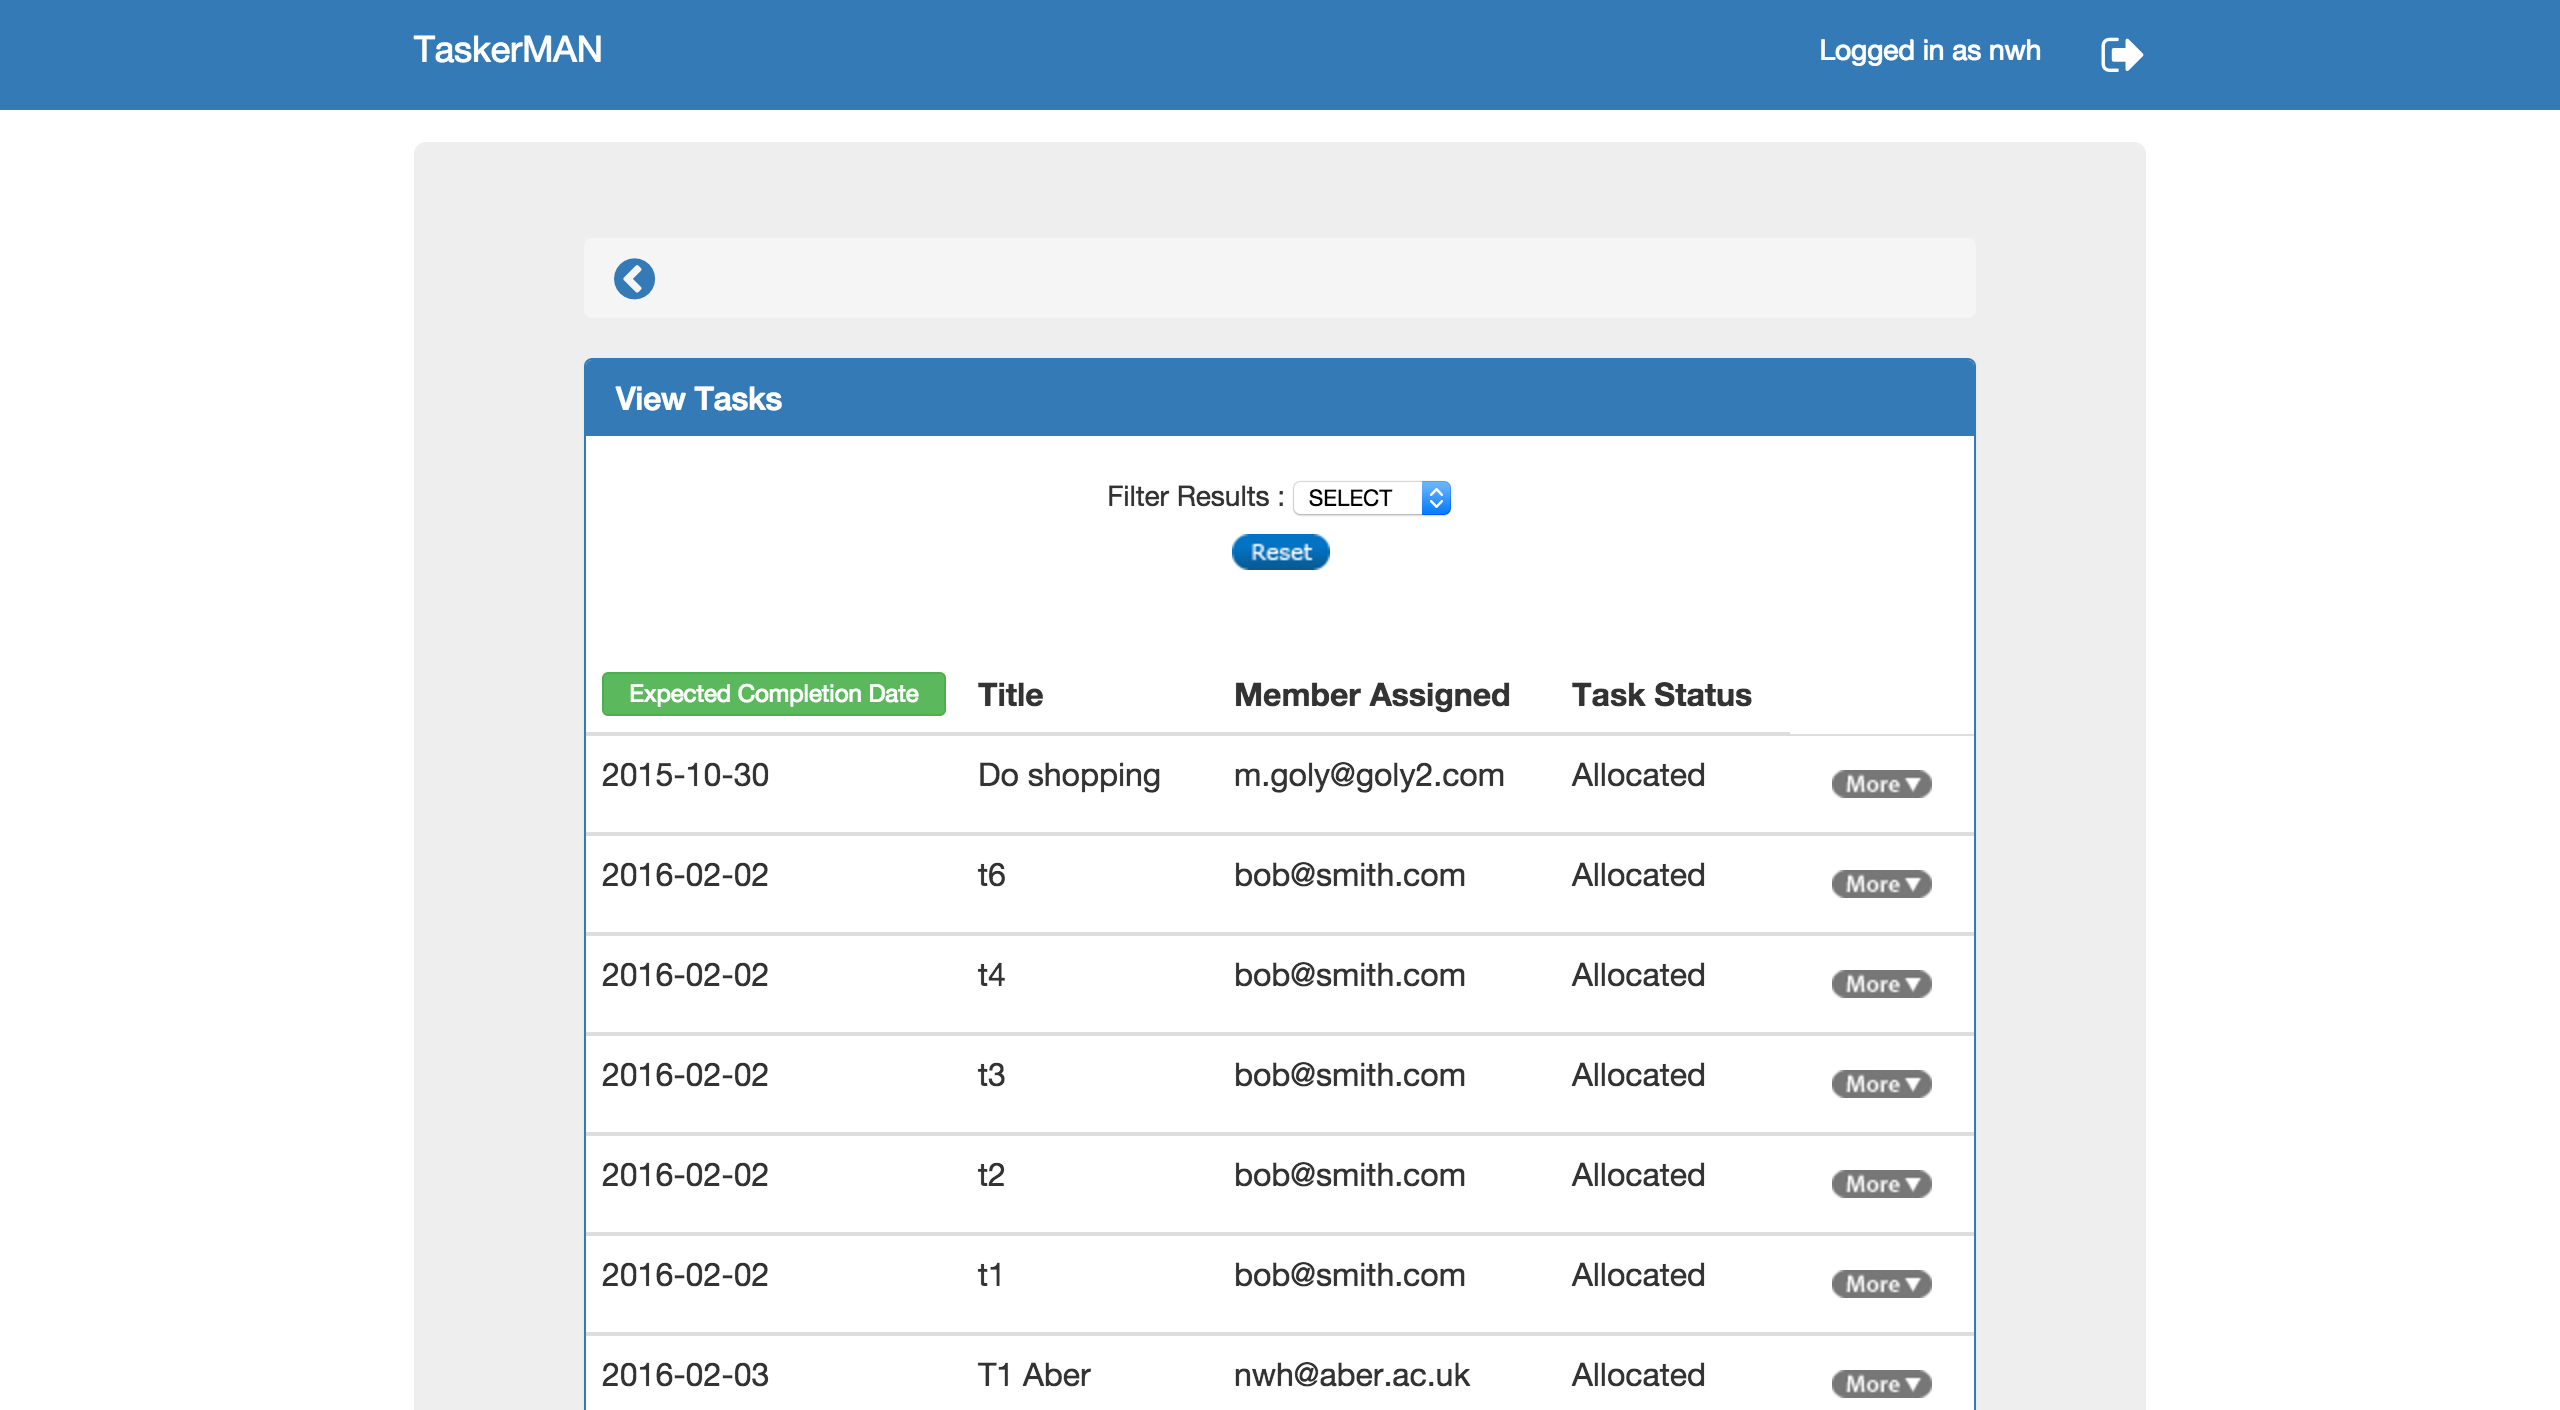
\includegraphics[width=0.75\textwidth, center]{images/5.2/TaskerMANViewTask} \\
This page shows all of the tasks that have been made, you can filter them by using the box at the top, for example by the name of the member, the date or the status. This web page helps you keep track easily of all of the tasks you have set. \\~\\
\underline{Other PHP Files - used for processing data} \\~\\
\underline{Adding a Task} \\~\\
One file used for processing data is the task.php file. This file firstly allows the user to enter in some information such as the start date of the task, completion date and member assigned. Then the information that is typed in, is processed using another PHP file which inserts what the user has typed in to the database, the file firstly connects to the database, checks the connection and then gets all the data the user typed in and adds it to the database. An if statement is then included to check that the data has been entered into the database correctly, if it has, the web page will display a message to the user confirming that a new task has been added to the database, then the user is presented with 3 options to add another task, log out or go back to the home page. If the data is not added to the database correctly due to a problem an error message will be printed out to the user and they won?t be able to go on any further in the process. \\~\\
\underline{Edit Tasks} \\~\\
The edittasks.php file presents the user with an area to modify the tasks they have set for example, changing who they have allocated the task to. This connects to the database and prints all of the relevant information in a table - all of the tasks are displayed at this point. From here the user can either update the task or delete the task. If they click on delete, a file called connectedb.php will run and depending on the id that it has (each record in the table has an id for reference purposes) it will then delete all the information from the task list via an SQL command and then closes the database connection. If the user selects the update option from the table they will be taken to a file called updatetask.php this once again is referenced using an ID and once the user clicks this button they are presented with all the information of the task, they can then update the description of the task, change the dates, change the status and member allocated.  To get this information, the user is connected to the database and a SELECT SQL query is used. Some text boxes are left open and if the information changes then the field is sent to the database that changes. Once you have updated the records, the user will be able to check their changes have been made by viewing all the tasks. If the update has been successful you will be presented with a confirmation message, if you have not, an error message will be displayed. If you have been successful you will have the option to update another record or go back to the home page. \\~\\
\underline{View Tasks} \\~\\
If you select this option from the home page you will be taken to a file called viewtasks.php. This web page pulls some information from the database using an SQL query to show all of the tasks and then it puts this information into a table to make it easier to read.  This webpage also includes a filter that allows the user to view the data based on the member or the status of the task. Once the user has looked at this information they can either log out or navigate back to the home page. \\~\\
\underline{Add User} \\~\\
If you select the add user option from the home page you will be presented with two text boxes described earlier in this document. Once you click the submit button you will be taken to a webpage called process1.php this just adds the information that the user has typed into the database via an SQL command. This once again has an if statement which if unsuccessful will provide the user with a simple error message, if successful in adding the user a confirmation will be shown and then the user will have a few navigation choices. \\~\\
\underline{Edit User} \\~\\
The editusers.php file presents the user with an area to modify their details if they have typed them in wrong or their details change. Currently the only fields we have here are name and email address. If the user wants to update these they just click on the update link and are then taken to an update.php page where they can then re-enter their name and email address. Once they have done that and are happy with it they click the update button which sends the new data they have put in to the database. They will then be provided with a confirmation message if it is successfully updated, and then you can navigate to other areas of the website. To make sure that the user types in information in the correct format we will be implementing some validation to check that the user is entering data of the correct type. Next you can go back to the editusers.php file and also delete records of users. This will be used for managers so that they can delete users from TaskerMAN if they need to. All that they need to do is look at the table of users that is provided in editusers.php and then click on the delete link of the user that they want to get rid of. Once they do that a confirmation message will be displayed telling them that the user has been successfully deleted. Once this action is completed by the user a file called connectdb.php runs which connects to the database is and then a delete SQL command is used to get rid of the user they deleted. Each user has a reference number, so this is what is used to delete a specific user. Next time they view the edit user's web page the table will have been updated to show all the users they want. To make sure users aren't accidentally deleted we should implement a pop up box to appear and make the user confirm that they want to delete a specific user. \\~\\
\underline{View Users} \\~\\
Once logged in, view users will enable you to look at all the people using the system - this tool will be used for managers only so they can view all the team members they can allocate tasks too. Once they have clicked on the view user's page, a table will be displayed - this will be populated with information about the users in the system (which will just be their name and email) and what tasks they have been allocated to do. To get this information, an SQL query will be used to select all the users and then this information is just output into a table. A filter could be used based on name, tasks allocated or another variable or we could sort the table so that it is in alphabetical order making it easier to find specific people or we could implement a search box. \\~\\
\section{Detailed Design}
\subsection{TaskerCLI Diagrams}
\subsection{TaskerMAN Diagrams}
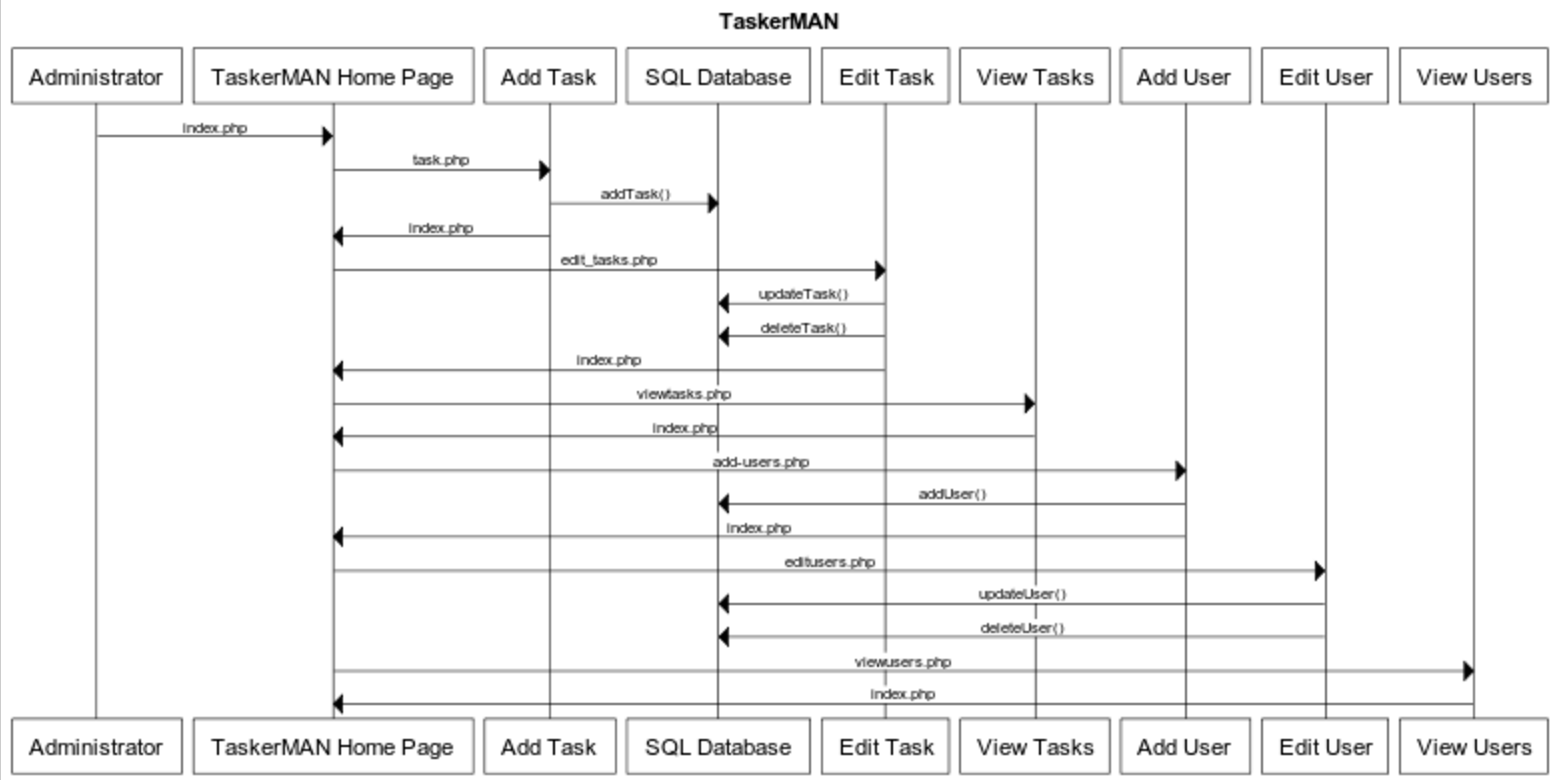
\includegraphics[width=1\textwidth, center]{images/Detailed-Design/TaskerMANSequenceDiagram} \\
\clearpage
\addcontentsline{toc}{section}{REFERENCES}
\begin{thebibliography}{12}
\bibitem{se.qa.ds} \emph{Software Engineering Group Projects}
Design Specification Standards.
C. J. Price, N.W.Hardy and B.P.Tiddeman, SE.QA.05A. 1.8 Release.
\bibitem{se.qa.rs} \emph{Software Engineering Group Projects}
Requirements Specifications.
N. W. Hardy, SE.QA.RS. 1.1 Release.
\bibitem{se.qa.rs fr8 local storage} \emph{Software Engineering Group Projects}
Requirements Specifications.
N. W. Hardy, SE.QA.RS, FR8 \emph{Local Storage of Tasks}. 1.1 Release.
\bibitem{se.qa.rs fr3} \emph{Software Engineering Group Projects}
Requirements Specifications.
N. W. Hardy, SE.QA.RS, FR3. 1.1 Release.
\bibitem{se.qa.rs fr4} \emph{Software Engineering Group Projects}
Requirements Specifications.
N. W. Hardy, SE.QA.RS, FR4. 1.1 Release.
\bibitem{se.qa.rs fr5} \emph{Software Engineering Group Projects}
Requirements Specifications.
N. W. Hardy, SE.QA.RS, FR5. 1.1 Release.
\bibitem{se.qa.rs fr6} \emph{Software Engineering Group Projects}
Requirements Specifications.
N. W. Hardy, SE.QA.RS, FR6. 1.1 Release.
\bibitem{se.qa.rs fr7} \emph{Software Engineering Group Projects}
Requirements Specifications.
N. W. Hardy, SE.QA.RS, FR7. 1.1 Release.
\bibitem{se.qa.rs fr8 user id} \emph{Software Engineering Group Projects}
Requirements Specifications.
N. W. Hardy, SE.QA.RS, FR8 \emph{User Identification}. 1.1 Release.
\bibitem{se.qa.rs fr11} \emph{Software Engineering Group Projects}
Requirements Specifications.
N. W. Hardy, SE.QA.RS, FR11. 1.1 Release.
\bibitem{se.qa.rs fr10} \emph{Software Engineering Group Projects}
Requirements Specifications.
N. W. Hardy, SE.QA.RS, FR10. 1.1 Release.
\bibitem{se.qa.rs ir1} \emph{Software Engineering Group Projects}
Requirements Specifications.
N. W. Hardy, SE.QA.RS, IR1. 1.1 Release.
\end{thebibliography}
\clearpage
\addcontentsline{toc}{section}{DOCUMENT HISTORY}
\section*{DOCUMENT HISTORY}
\begin{tabular}{|l | l | l | p{8cm} |l | }
\hline
Version & CCF No. & Date & Changes made to Document & Changed by \\
\hline
1.0 & N/A & 2015-10-27 & Initial creation for review & L. Jones \\
\hline
1.1 & N/A & 2015-10-28 & Updated the TaskerCLI user interface section & M. Goly \\
\hline
1.2 & N/A & 2015-10-28 & Created sub-subsections for  Use-cases and User-interface design & L. Jones \\
\hline
1.3 & N/A & 2015-10-29 & Added TaskerCLI Use-Case diagram and narrative & L. Jones \\
\hline
1.4 & N/A & 2015-10-29 & Updated version from review to release & L. Jones \\
\hline
1.5 & N/A & 2015-11-24& Added Sections for Design Specification Review & L. Jones \\
\hline
\end{tabular}
\label{thelastpage}
\end{document}
\end{verbatim}
\label{fig:footer}
\end{figure}
\label{thelastpage}
\end{document}
